W wyniku testów wyłoniony został model o~najlepszej dokładności realnej, tj.
dokładności klasyfikacji zewnętrznych grafów testowych.
Model ten okazał się jednym z~najbardziej podstawowych z~przygotowanych,
bo jest to podstawowy model uczony na grafach sześciowierzchołkowych.
W ramach eksperymentu, zastosowano dla niego modyfikacje,
które pomogły zwiększyć realną dokładność modelu.
Modyfikacje te zostały wprowadzone i~przetestowane w~podrozdziale z~testami modeli
z walidacją krzyżową.
Jedyną zmianą z~zaproponowanych, która przynosi realne korzyści,
jest zwiększenie liczby filtrów w~warstwach sieci neuronowej, kolejno 32, 64 oraz 128 dla Conv2D,
oraz zastosowanie zwiększonego parametru dropout - 0,5.

\subsubsection{Zmodyfikowany model podstawowy uczony na grafach sześciowierzchołkowych}

Model osiąga wysokie i~stabilne wyniki, lecz po około 55 epoce procesu nauczania,
dokładność gwałtownie spada, aż do wartości około 23\%.

Ta sama sytuacja dotyczy straty, która to gwałtownie wzrasta około 60 epoki,
z około 0,25, do aż 1,75.

\begin{figure}[ht]
	\centering
	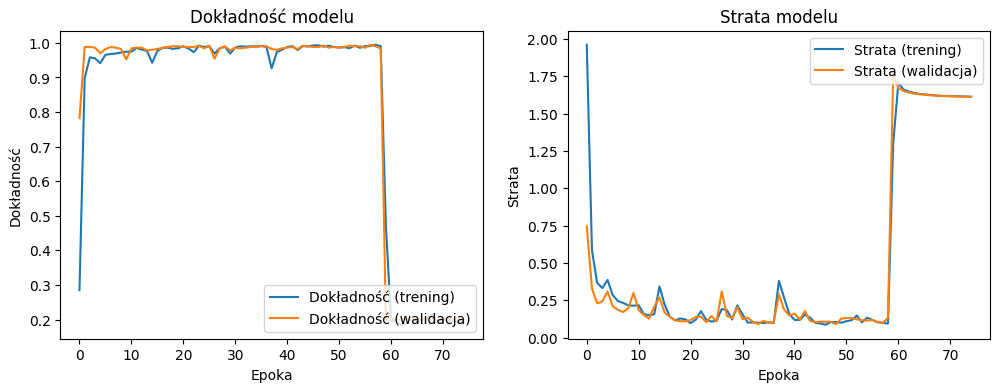
\includegraphics[height=5.5cm]{resources/tests/images/v4/base6_1_img.png}
	\caption{Wyniki testów dla zmodyfikowanego modelu podstawowego, liczba wierzchołków n = 6}
	\label{Fig:tests-best-0a}
\end{figure}
\FloatBarrier

Powyższa sytuacja wskazuje na poważny problem z~wydajnością modelu,
np. przetrenowanie lub problem techniczny w~procesie treningu
- być może był to zbyt niski współczynnik procesu uczenia,
który spowodował, że model „przyspieszył” w~ostatnich epokach.

% \begin{figure}[ht]
% 	\centering
% 	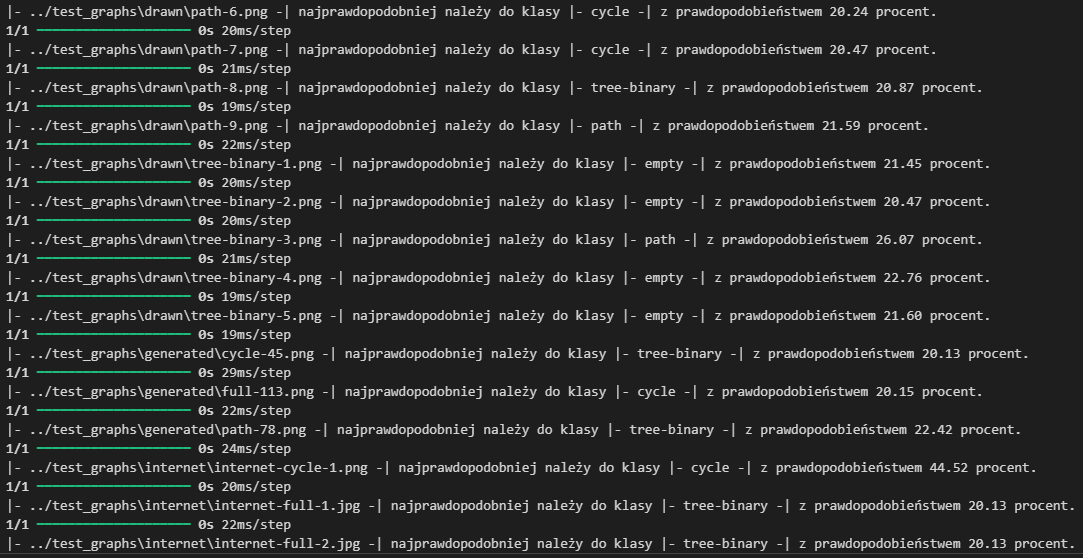
\includegraphics[width=14cm]{resources/tests/images/v4/base6_1_txt.png}
% 	\caption{Klasyfikacja obrazów zewnętrznych dla zmodyfikowanego modelu podstawowego, liczba wierzchołków n = 6}
% 	\label{Fig:tests-base-5b}
% \end{figure}
% \FloatBarrier

% \begin{figure}[ht]
% 	\centering
% 	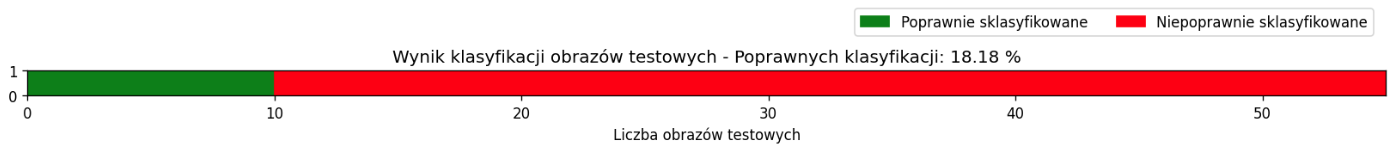
\includegraphics[width=14cm]{resources/tests/images/v4/base6_1_bar.png}
% 	\caption{Wizualizacja klasyfikacji obrazów zewnętrznych dla zmodyfikowanego modelu podstawowego, liczba wierzchołków n = 6}
% 	\label{Fig:tests-base-5c}
% \end{figure}
% \FloatBarrier

\subsubsection{Zmodyfikowany poprawiony model podstawowy uczony na grafach sześciowierzchołkowych}

Wyniki uzyskane z~procesu nauki poprzeniego modelu sugerują zmniejszenie liczby epok do około 55.
Taka modyfikacja została zastosowana, a~test przeprowadzono ponownie.

Po skróceniu procesu uczenia, dokładność modelu nie spada gwałtownie w~końcowych epokach.
Dokładność szybko rośnie na początku treningu i~osiąga wysokie wartości już po kilku epokach.
Dokonuje się również stabilizacja w~okolicach 98\%-100\%, co wskazuje na dobre dopasowanie modelu do danych.
Fluktuacje walidacji są niewielkie i~nie wskazujące na problemy z~modelem.

Strata, po modyfikacji, już nie wzrasta gwłatownie pod koniec procesu uczenia.
Oba typy strat maleją po kilku pierwszych epokach i~pozostają na niskim poziomie (0,1 - 0,2).
Model wygląda więc na dobrze dopasowany do danych treningowych, jak i~walidacyjnych.

\begin{figure}[ht]
	\centering
	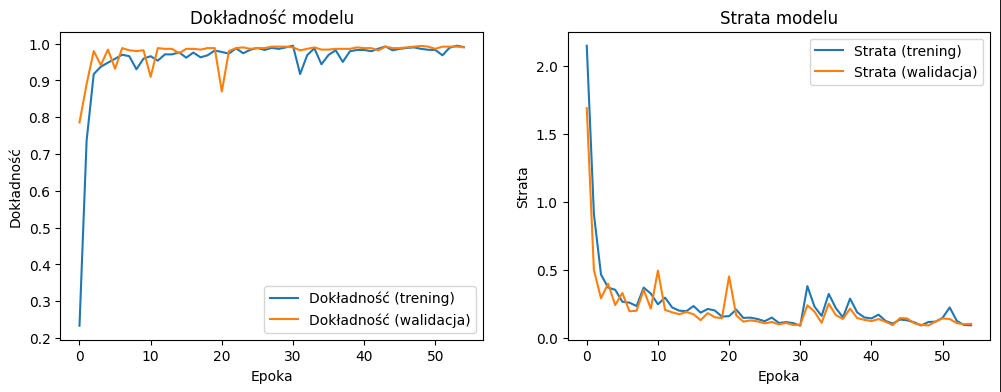
\includegraphics[height=5.5cm]{resources/tests/images/v4/base6_1_1_img.png}
	\caption{Wyniki testów dla poprawionego zmodyfikowanego modelu podstawowego, liczba wierzchołków n = 6}
	\label{Fig:tests-best-1a}
\end{figure}
\FloatBarrier

Wygląda na to, że model efektywnie klasyfikuje grafy ze zbioru walidacyjnego.
Zwracając uwagę na powyższe wskaźniki, można spodziewać się dobrej jakości przewidywań.
Model działa bardzo dobrze, z~minimalnymi fluktuacjami, które mogą być naturalne przy tego typu zadaniach.

\begin{figure}[ht]
	\centering
	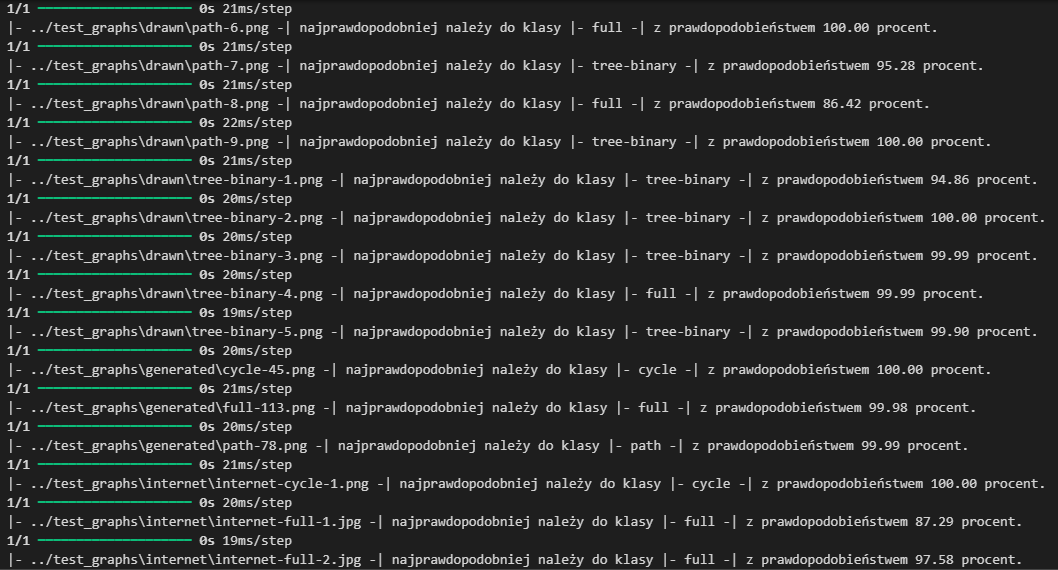
\includegraphics[width=14cm]{resources/tests/images/v4/base6_1_1_txt.png}
	\caption{Klasyfikacja obrazów zewnętrznych dla poprawionego zmodyfikowanego modelu podstawowego, liczba wierzchołków n = 6}
	\label{Fig:tests-best-2b}
\end{figure}
\FloatBarrier

\begin{figure}[ht]
	\centering
	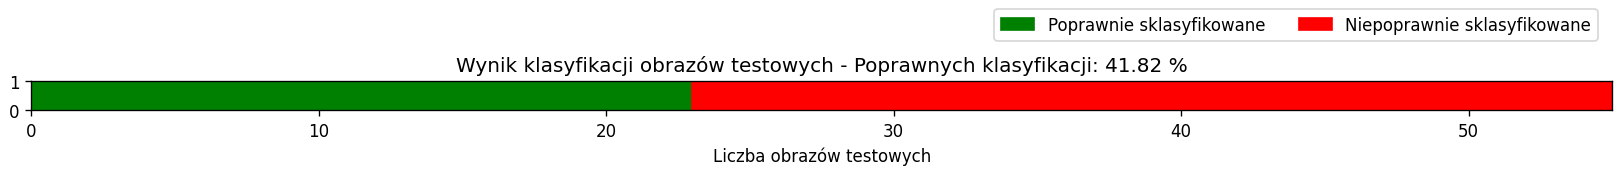
\includegraphics[width=14cm]{resources/tests/images/v4/base6_1_1_bar.png}
	\caption{Wizualizacja klasyfikacji obrazów zewnętrznych dla poprawionego zmodyfikowanego modelu podstawowego, liczba wierzchołków n = 6}
	\label{Fig:tests-best-1c}
\end{figure}
\FloatBarrier

Zmodyfikowany model poprawnie sklasyfikował prawie 42\% grafów zewnętrznych.
Jest to wynik gorszy o~3 punkty procentowe od wariantu tego samego modelu
z mniejszą liczbą filtrów w~warstwach Conv2D oraz niższym wskaźnikiem dropout.
Wynik jednak jest wciąż zadowlający, bo czterdziestodwuprocentowa pewność,
jest wynikiem lepszym niż przypisywanie klas losowo.

\begin{figure}[ht]
	\centering
	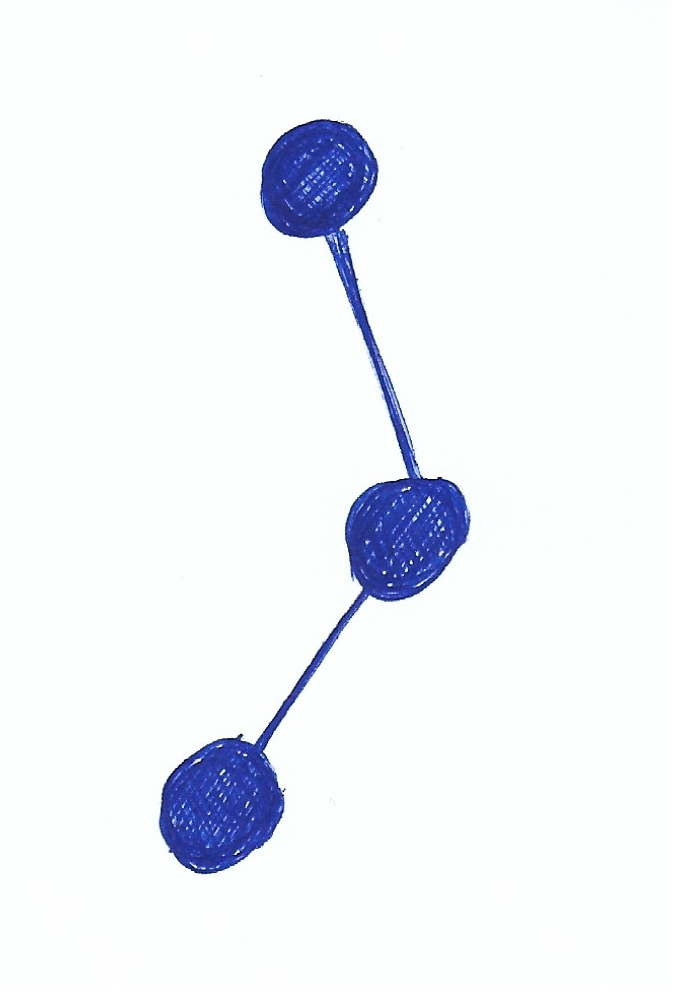
\includegraphics[width=10cm]{../graph_classification/test_graphs/drawn/path-4.png}
	\caption{Klasyfikacja przykładowego grafu zewnętrznego przez zmodyfikowany poprawiony model podstawowy
		uczony na grafach sześciowierzchołkowych
		Przypisana klasa to drzewo binarne z~100\% pewnością.}
	\label{Fig:tests-best-1d}
\end{figure}
\FloatBarrier

Ponownie, to prostszy model okazał się tym, który dokonuje lepszej generalizacji na nowe dane
i lepiej zapamiętuje ogólne wzorce.
Sugeruje to, że zbyt duże skomplikowanie modelu do zadania o~niewielkiej złożoności,
przynosi korzyści odwrotne od zamierzonych.